\chapter{問題提起と文献調査}
\label{related_works}

本章では、研究背景について問題提起の形で示し、その上でリサーチクエスチョンを提示する。また、その問いを探索する切り口として本研究が着目した「手指の変換」について、その観点から取り組む動機、そして関連研究との相違点を説明することから研究の位置付けを明らかにする。

% \section{Gallagherのミニマルセルフ}


% こうした研究で蓄積された実証的知見は、インターフェースデザインや身体拡張の設計・評価へと応用されている。インターフェース研究者の渡邊は、機械や情報処理が介在する高度で複雑な道具であっても、「使っている最中にはその道具自体を意識せずに身体の一部になったかのようになり、目的に集中できる」こと、すなわち「道具の透明化」という、ヒューマンインターフェースの理想を実現するための指針としてこの概念に注目する。渡邊は、例えばマウスカーソルやスマートフォンのような「操作時の指とグラフィックの追従性が高い」インターフェースには「自己帰属感(Gallagherのsense of ownershipに対する訳語)」が生じるとし、このことからこうしたインターフェースは「自身の一部、延長」として考えられ、「道具の透明化」が実現すると説明する\cite{Watanabe2013}\cite{Watanabe2017}。

\section{FelsのEmbodiment}
前節で触れた、FelsのEmbodimentに関する分類をここで詳しく説明する。
Sydney Felsは、対象と人との関係性について、Reponse、Control、Gontemplation、Belongingの4つに分類した\cite{Fels, Costello2005}。それぞれの説明は以下の通りである(括弧内は筆者が訳語を当てた)。

\textbf{Response(応答):}\\
対象に対する働きかけの結果から、感情的な反応や理解を得る状態を指す。Felsはこの関係性の例として「コンピュータとそれに初めて触れた人」を挙げ、「なんらかの操作を通して得られた、便利な機能に喜んでいる状態、また逆に「有用な結果を得られず落胆する状態」と説明する。

\textbf{Control(制御):}\\
人が対象を自分自身の延長として使用し、その操作によって感情的な満足や美的体験を得る状態を指す。例えばピアノの演奏において、「音が出ている」ということだけでなく、自分自身の表現したいことが、不自由なくピアノを通して体現されていると感じるときの、一体感によってもたらされる心地よさがこれに該当する\footnote{「Control」においてFelsは、「自分自身の延長」として経験される感覚であり、またそれが追従性の高いグラフィックによってもたらされると説明する。これは、渡邊がマウスカーソルやスマートフォンに対して用いた「操作時の指とグラフィックの追従性が高い」インターフェースという説明と同等のものであると考えられる。このことからFelsのいうControlとは、Gallagherの「sense of ownership」と重なる。}。

\textbf{Contemplation(鑑賞):}\\
人が対象に対して働きかけることはないが、人がその対象からの信号やメッセージを内省や反映を通じて、感情的になったり美的体験を得る状態を指す。Felsはその具体例として、絵画の鑑賞体験を挙げる。

\textbf{Belonging(帰属):}\\
対象によって人が動かされているような経験を指す。人はその対象によって提供される体験を通じて感情的な反応を得る。ここでは、対象が人の体験や感情を形作る役割を果たす。たとえばバイクの運転において、「バイクに合わせた走り方をする」といったように、単にその対象を通して使い手の意図がそのまま体現されるのではなく、その対象に合わせた振る舞いがそこで形作られることに喜びを見出すような状態である。

\begin{figure}[H]
  \centering
  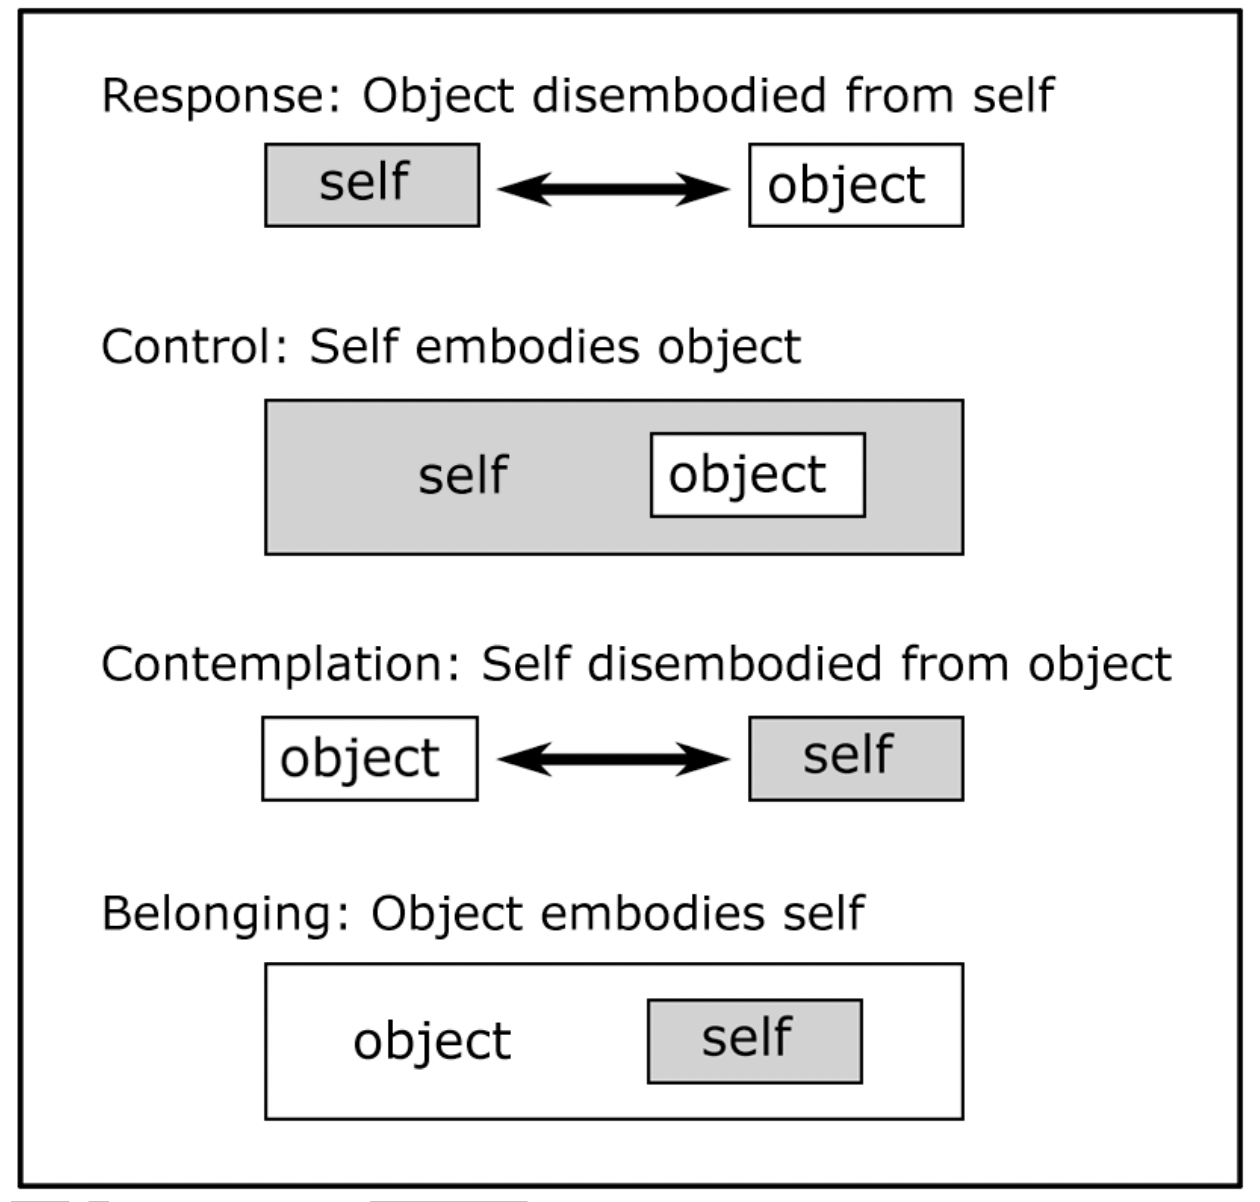
\includegraphics[width=8cm]{img/fels_diagram.png}
  \caption{FelsによるEmbodiment(仮置き)}
  \label{fig:fels_embodiment}
\end{figure}

% さて、Felsは特に、上記「制御 Control」においては「自分自身の延長」として経験される感覚について言及しており、またそれが追従性の高いグラフィックによってもたらされるという記述は、渡邊がマウスカーソルやスマートフォンに対して用いた「操作時の指とグラフィックの追従性が高い」インターフェースという説明と同等のものである。このことからFelsのいうControlとは、Gallagherの「sense of ownership」と同じものを指していると考えられる。その上で、Embodimentの状態をControlのみならずBelongingから捉えていること、そしてEmbodimentが生じていない状態についても言及していることなど、現在HCIの分野で一般に用いられる意味でのEmbodimentよりも広く、人と対象を捉えるモデルとなっていることが確認できる。

% さらにFelsは、対象と人とのあいだにある「深い関係」を指して、「Intimacy」という尺度で説明する。例えば楽器と人の関係性ように、Intimacyのある関係性のもとでは、「あたかもその装置が身体の延長であるかのように、考えや感情を効果的に表現できる」という。上記の、FelsによるEmbodimentの分類においては、ResponseがIntimacyの低い状態、ControlがIntimacyの高い状態として説明される。

前節で指摘した「対象に自己が歩み寄っていく」ことを通して得られる一体感とは、Felsの分類におけるBelongingである。しかし、Belongingのような一体感を抱いている状態であっても、人が対象に向けて「Control」することも同時に行われている。このように、自分の意志と対象の制約や他者性とのあいだで折り合いをつけることで得られる「親密な関係」を、Felsは「Intimacy」という言葉で説明した。

\section{身体の変換や拡張を扱う先行事例(執筆中)}
身体の変換や拡張を行う研究は近年、数多く行われている\footnote{近年に多いとする根拠は、小鷹の「ラバーハンド錯覚の遅い発見問題」という問題意識に基づく。小鷹は、「ラバーハンド錯覚」というシンプルな錯覚が学術的にはじめて発表されたのが1998年と遅く、それが「コンピュータの普及により、事物を情報的に処理する感受性が世界に浸透しつつあった1990年代後半」であったことに、単なる偶然ではない「情報としての身体」という発想を後押しするものがあったのではないかと指摘する\cite{kodaka}。}\cite{Kondo2020, ekusute,Kasahara2017,augmented_hand_series}。

小川らによる「えくす手(Metamorphosis Hand)」\cite{ekusute}では、指の伸びた手などの現実の身体にはあり得ない特性を持ったバーチャルな身体を通じてピアノを演奏することができる。そのねらいは、「現実とは異なる特性のバーチャルハンドへの身体所有感の生起を通じ、現実の身体的制約を超えたインタラクションを実現する、一種のバーチャルな身体拡張体験を提供する」と説明される。

身体所有感の生起要因に関するこれまでの議論を参照し、本作は「テクスチャ、形状、空間的配置、解剖学的構造の4つの特性」を根拠に、身体所有感が生じながらも、自己身体と意味的に類似しないバーチャルハンドを制作している。これらの特性は、身体所有感を生じさせる上での実証的知見ではあるが、本研究が対象とするIntimacyは、例えば楽器のように、こうした生起要因を押さえなくとも、習得を経て生じうるのではないかと考える。また、生起要因を多く踏襲しているわけではないからこそ、身体所有感が生じるまでには期間を必要とし、その程度にも個人差が生じるのではないだろうか。これらの観点から、本研究の取り組みは「えくす手」よりも極端な身体変容を促す体験として位置付けられる。

Golan Levinによる「Augmented Hand Series」\cite{augmented_hand_series}は、

佐藤雅彦らによる「君の身体を変換してみよ展」はさまざまなアプローチで身体の変容を扱う作品が展示されたが、その中でも《点にんげん・線にんげん》\cite{sato_icc}という作品は、ボディトラッキングを用いて取得された全身の関節の位置を捉えたキーポイントが点として扱われ、異なる方法で結びつけられたり、ボロノイ分割が適用される点群として扱われるなど、さまざまな「変換」が行われている。\\
本作品との構造上の相違点として、関節の位置を捉えたキーポイントの並び替えの有無が挙げられる。佐藤らの作品では、身体の関節の位置を捉えたキーポイントはその配置を変えることなく、繋げ方やインターフェースの文脈における位置付けの違いで展開される。一方、本作ではキーポイントの配列もダイナミックに変化する。これは、手指が複雑な動きのできる器官であると同時に、身体の中でもっとも随意に動かすことのできる器官でもあることから、構造が大きく異なる場合でも、手指の動きに連動している箇所を、動かしている中で容易に同定できると考えているためである。


